\documentclass[12pt, titlepage]{article}

\usepackage{amsmath, mathtools}

\usepackage[round]{natbib}
\usepackage{amsfonts}
\usepackage{amssymb}
\usepackage{graphicx}
\usepackage{colortbl}
\usepackage{xr}
\usepackage{hyperref}
\usepackage{longtable}
\usepackage{xfrac}
\usepackage{tabularx}
\usepackage{float}
\usepackage{siunitx}
\usepackage{booktabs}
\usepackage{multirow}
\usepackage[section]{placeins}
\usepackage{caption}
\usepackage{fullpage}

\hypersetup{
bookmarks=true,     % show bookmarks bar?
colorlinks=true,       % false: boxed links; true: colored links
linkcolor=red,          % color of internal links (change box color with linkbordercolor)
citecolor=blue,      % color of links to bibliography
filecolor=magenta,  % color of file links
urlcolor=cyan          % color of external links
}

\usepackage{array}

\externaldocument{../../SRS/SRS}


\title{Module Interface Specification for SmartLock \progname{}}

\author{\authname}

\date{\today}

%% Comments
\usepackage{color}
\newif\ifcomments\commentstrue %displays comments
%\newif\ifcomments\commentsfalse %so that comments do not display
\ifcomments
\newcommand{\authornote}[3]{\textcolor{#1}{[#3 ---#2]}}
\newcommand{\todo}[1]{\textcolor{red}{[TODO: #1]}}
\else
\newcommand{\authornote}[3]{}
\newcommand{\todo}[1]{}
\fi
\newcommand{\wss}[1]{\authornote{blue}{SS}{#1}} 
\newcommand{\plt}[1]{\authornote{magenta}{TPLT}{#1}} %For explanation of the template
\newcommand{\an}[1]{\authornote{cyan}{Author}{#1}}
%% Common Parts
\newcommand{\progname}{4TB6 - Mechatronics Capstone} % PUT YOUR PROGRAM NAME HERE
\newcommand{\authname}{Team \#5, Locked \& Loaded
\\ Abi Nevo, nevoa
\\ Elsa Bassi, bassie
\\ Steffi Ralph, ralphs1
\\ Abdul Iqbal, iqbala18
\\ Stephen De Jong, dejons1
\\ Anthony Shenouda, shenoa2} % AUTHOR NAMES                  

\usepackage{hyperref}
    \hypersetup{colorlinks=true, linkcolor=blue, citecolor=blue, filecolor=blue,
                urlcolor=blue, unicode=false}
    \urlstyle{same}


\begin{document}
\maketitle
\thispagestyle{empty}
%\begin{figure}[h!]
%  \centering
 % 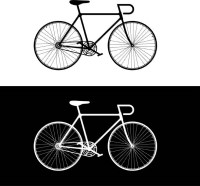
\includegraphics[width=0.4\linewidth]{../BikeLogo.jpg}
%\end{figure}

\newpage
\pagenumbering{roman}
\begin{table}[hp]
\caption{Revision History} \label{TblRevisionHistory}
\begin{tabularx}{\textwidth}{llX}
\toprule
\textbf{Date} & \textbf{Developer(s)} & \textbf{Change}\\
\midrule
16-01-23 & Abi & Started M4, M5, M7\\
17-01-23  & Abi & Finished M4, M5, M7, Intro\\
18-01-23 & Anthony & Finished M2,3,6,8\\
07-04-23 & Abi and Anthony & Rev 1 updates\\
\bottomrule
\end{tabularx}
\end{table}


\newpage
\tableofcontents
\listoftables

\newpage
\pagenumbering{arabic}

\section{Symbols, Abbreviations and Acronyms}

See SRS Documentation \href{https://github.com/NevoAbigail/Capstone/blob/main/docs/SRS/SRS.pdf}{here}.

%\wss{Also add any additional symbols, abbreviations or acronyms}

\section{Introduction}

The following document details the Module Interface Specifications for
SmartLock, a bluetooth-driven bike lock brough to you by the Locked \& Loaded team. The SmartLock allows users to unlock their bike remotely using Bluetooth. 

%\wss{Fill in your project name and description}

Complementary documents include the System Requirement Specifications
and Module Guide.  The full documentation and implementation can be
found in \href{https://github.com/NevoAbigail/Capstone}{the GitHub repo}. % \wss{provide the url for your repo}

Note that not every module documented in the Module Guide has a corresponding section in this document, as an MIS was only completed for every software module, and not those modules with a hardware implementation. 

\section{Notation}

\progname \ uses functions, which
are defined by the data types of their inputs and outputs. Local functions are
described by giving their type signature followed by their specification.

\section{Module Decomposition}

The following table is taken directly from the \href{https://github.com/NevoAbigail/Capstone/blob/main/docs/Design/SoftArchitecture/MG.pdf}{Module Guide document} for this project.

\begin{table}[h!]
\centering
\begin{tabular}{p{0.3\textwidth} p{0.6\textwidth}}
\toprule
\textbf{Level 1} & \textbf{Level 2}\\
\midrule

\multirow{2}{0.3\textwidth}{Hardware-Hiding Module} & User Input to Phone Module \\
& Solenoid Actuation Module \\
\midrule

\multirow{6}{0.3\textwidth}{Behaviour-Hiding Module} %& Engage Status Signal Module  \\
& Arduino Bluetooth Communication Module\\
& Mobile App Bluetooth Communication Module\\
& Battery Status Module \\
& Location Module  \\
& Lock Frame Module \\
\midrule

\multirow{5}{0.3\textwidth}{Software Decision Module} & User Disengage Module \\
& Hardware Disengage Module \\
& Battery Module \\
& Locking Mechanism Module \\
\bottomrule

\end{tabular}
\caption{Module Hierarchy}
\label{TblMH}
\end{table}

\newpage




\section{MIS of Arduino Bluetooth Communication Module} \label{mABC}

\subsection{Module}
disengageControl.ino

\subsection{Syntax}

\subsubsection{Exported Constants}

\begin{center}
\begin{tabular}{p{4cm} p{2cm} p{6cm}}
\hline
\textbf{Name} & \textbf{Value} & \textbf{Description} \\
\hline
BAUD\_RATE & 9600 & Serial communication baud rate \\
GREEN\_PIN & 23 & Pin for green LED onboard \\
\hline
\end{tabular}
\end{center}

\subsubsection{Exported Access Programs}

\begin{center}
\begin{tabular}{p{2cm} p{2cm} p{2cm} p{2cm} p{5cm}}
\hline
\textbf{Name} & \textbf{In} & \textbf{Transition} & \textbf{Out} & \textbf{Exception} \\
\hline
setup & None & loop & None & BLE fails: print message  \\
loop & None & \hyperref[mHD]{Hardware Disengage Module} & None & BLE fails: print message \\
\hline
\end{tabular}
\end{center}

\subsection{Semantics}

\subsubsection{State Variables}

\begin{center}
\begin{tabular}{p{4cm} p{4cm} p{6cm}}
\hline
\textbf{Name} & \textbf{Type} & \textbf{Description} \\
\hline
nanoService & BLEService & BLE service UUID\\
commCharacteristic & BLEByteCharacteristic & BLE Characteristic UUID\\
password & int & password for disengage \\
productName & char array & name to appear when device BL advertised \\
central & BLEDevice & connected central device \\
\hline
\end{tabular}
\end{center}

\subsubsection{Access Routine Semantics}

\noindent setup
\begin{itemize}
\item Begins serial communication operating at BAUD\_RATE
\item Configures output pins specified by Exported Constants
\item Configures BLE settings: name, advertising service, characteristic, and initial value for the characteristic. Do this using functions from the Arduino Bluetooth library, use  \textit{\#include ArduinoBLE.h}
\item Begins advertising BL service, and awaits for connections, prints status message

\end{itemize}

\noindent loop
\begin{itemize}
\item Listens for central device to connect using aforementioned Bluetooth library
\item If a central device is connected, print a statement of this status and transition to \hyperref[mHD]{Hardware Disengage Module}
\item When the central device disconnects, print a message indicating this new status
\end{itemize}

\subsubsection{Local Functions}

A list of functions used in this module from Arduino Bluetooth library, \href{https://www.arduino.cc/reference/en/libraries/arduinoble/}{see official Arduino documentation here}
\begin{itemize}
    \item setDeviceName()
    \item setLocalName()
    \item setAdvertisedService()
    \item addCharacteristic()
    \item addService()
    \item writeValue()
    \item advertise()
\end{itemize}


%%END OF ARDUINO BLUETOOTH COMM MODULE



\section{MIS of Hardware Disengage Module} \label{mHD}

\subsection{Module}
disengageControl.ino

\subsection{Syntax}

\subsubsection{Exported Constants}

\begin{center}
\begin{tabular}{p{4cm} p{2cm} p{6cm}}
\hline
\textbf{Name} & \textbf{Value} & \textbf{Description} \\
\hline
BAUD\_RATE & 9600 & Serial communication baud rate \\
GREEN\_PIN & 23 & Pin for green LED onboard \\
TRANSISTOR\_OUT & 9 & Output pin for signal to transistor \\
\hline
\end{tabular}
\end{center}

\subsubsection{Exported Access Programs}

\begin{center}
\begin{tabular}{p{2cm} p{2cm} p{4cm} p{2cm} p{2cm}}
\hline
\textbf{Name} & \textbf{In} & \textbf{Transition} & \textbf{Out} & \textbf{Exception} \\
\hline
setup & None & loop & None & - \\
loop & None & see Access Routine Semantics & None & -\\
\hline
\end{tabular}
\end{center}

\subsection{Semantics}

\subsubsection{State Variables}

\begin{center}
\begin{tabular}{p{4cm} p{4cm} p{6cm}}
\hline
\textbf{Name} & \textbf{Type} & \textbf{Description} \\
\hline
password & int & password for disengage \\
central & BLEDevice & connected central device \\
commCharacteristic & BLEByteCharacteristic & BLE Characteristic UUID\\
\hline
\end{tabular}
\end{center}

\subsubsection{Access Routine Semantics}

\noindent setup
\begin{itemize}
\item Begins serial communication operating at BAUD\_RATE
\item Configures output pins specified by Exported Constants
\end{itemize}

\noindent loop
\begin{itemize}
\item While a central device is connected;
\item If the central device writes a value to the Arduino;
\item If the written value matches \textit{password};
\item Then print a message indicating this status, turn on the onboard green LED (write a LOW signal to GREEN\_PIN, and write a HIGH signal to TRANSISTOR\_OUT;
\item Else, turn off the onboard green LED (write a HIGH signal to GREEN\_PIN, and write a LOW signal to TRANSISTOR\_OUT;
\item This logic can also be described formally, using discrete math, with the following:

If the central device is connected:
$$central = C = \text{True}$$

If the central device writes a value to the Arduino:
$$commCharacteristic.written() = W = \text{True}$$

If the written value matches \textit{password}:
$$P = \text{True}$$

If $P$ is true, then print a message indicating the status, turn on the onboard green LED, and set the transistor output high:
$$P \Rightarrow (GREEN\_PIN = \text{LOW} \land TRANSISTOR\_OUT = \text{HIGH})$$

If $P$ is false, then turn off the onboard green LED, and set the transistor output low:
$$P \Rightarrow (GREEN\_PIN = \text{HIGH} \land TRANSISTOR\_OUT = \text{LOW})$$
\end{itemize}

\subsubsection{Local Functions}

No local functions.


%%END OF HARDWARE DISENGAGE


\section{MIS of Mobile App Bluetooth Communication and User Disengage Module} \label{mHD}

\subsection{Module}
device.dart

\subsection{Semantics}

\subsubsection{State Variables}

\begin{center}
\begin{tabular}{p{4cm} p{4cm} p{6cm}}
\hline
\textbf{Name} & \textbf{Type} & \textbf{Description} \\
\hline
locking & int & request to engage the lock (value of 1 to engage) \\
isConnected & int & whether SmartLock App is connected to the Arduino (value of 1 if connected) \\
password & int & the value of the user inputted password \\
\hline
\end{tabular}
\end{center}

\subsubsection{Local Functions}

\noindent buildServiceTiles
\begin{itemize}
\item Constructs the layout of the screen displaying the connected device
\item Configures the buttons to disengage lock by sending the user inputted password to the Arduino 
\end{itemize}

\begin{itemize}
\item inputs: password
\item transition: none
\item output: password to Arduino
\item exception: none
\end{itemize}

\noindent Widget build (BuildContext context)
\begin{itemize}
\item Constructs the layout of the screen displaying the bluetooth devices
\item Displays the connection status of the selected bluetooth device
\end{itemize}

\begin{itemize}
\item inputs: none
\item transition: none
\item output: connection status displayed to user and device information
\item exception: none
\end{itemize}
% End of Mobile App Bluetooth Communication Module

\section{MIS of Battery Status Module} \label{mHD}

\subsection{Module}
main.dart

\subsection{Semantics}

\subsubsection{State Variables}

\begin{center}
\begin{tabular}{p{4cm} p{4cm} p{6cm}}
\hline
\textbf{Name} & \textbf{Type} & \textbf{Description} \\
\hline
batteryPercentage & int & the calculated value of the battery percentage \\
completedActuations & int & the total number of actuations to engage the lock completed \\
\hline
\end{tabular}
\end{center}

\subsubsection{Local Functions}

\noindent getLocalPath
\begin{itemize}
\item This functions gets the local directory of the application
\end{itemize}

\noindent getLocalFile
\begin{itemize}
\item This function gets the local file that stores the battery percentage and number of completed actuations 
\item It searches for a file called 'batteryInfo.txt'
\end{itemize}

\noindent writeBattery
\begin{itemize}
\item This function reads the value of the calculated battery percentage from the 'batteryInfo.txt' file
\end{itemize}

\noindent readBattery
\begin{itemize}
\item This function writes the value of the calculated battery percentage to the 'batteryInfo.txt' file
\item If this file can not be found (if this the first time the application is run) it will create a new file titled 'batteryInfo.txt'
\end{itemize}

\noindent batteryCalculator
\begin{itemize}
\item This function is used to calculate the amount of battery remaining
\item This is done by dividing the total capacity of the battery by the power drawn from completing on actuation of engaging the lock: \newline $\text{Battery Life} = \frac{\text{Total Capacity of Battery}}{\text{Power Drawn from Completing One Actuation of Engaging the Lock}}$
\end{itemize}

\begin{itemize}
\item inputs: batteryPercentage
\item transition: none
\item output: new battery percentage
\item exception: none
\end{itemize}

%% END OF BATTERY STATUS MODULE

\section{MIS of Location Module} \label{mHD}

\subsection{Module}
currentLocation.dart

\subsection{Semantics}

\subsubsection{State Variables}

\begin{center}
\begin{tabular}{p{4cm} p{4cm} p{6cm}}
\hline
\textbf{Name} & \textbf{Type} & \textbf{Description} \\
\hline
locLAT & double & the latitude coordinates of the users current location \\
locLOG & double & the longitude coordinates of the users current location \\
\hline
\end{tabular}
\end{center}

\subsubsection{Local Functions}

\noindent getLocalPath
\begin{itemize}
\item This functions gets the local directory of the application
\end{itemize}

\noindent getLocalFileLat
\begin{itemize}
\item This function gets the local file that stores the latitude coordinates
\item It searches for a file called 'locationLat.txt'
\end{itemize}

\noindent getLocalFileLog
\begin{itemize}
\item This function gets the local file that stores the longitude coordinates
\item It searches for a file called 'locationLog.txt'
\end{itemize}

\noindent readLat
\begin{itemize}
\item This function reads the value of the latitude coordinates from the 'locationLat.txt' file
\item If this file can not be found (if this the first time the application is run) it will create a new file titled 'locationLat.txt'
\end{itemize}

\noindent readLog
\begin{itemize}
\item This function reads the value of the longitude coordinates from the 'locationLog.txt' file
\item If this file can not be found (if this the first time the application is run) it will create a new file titled 'locationLog.txt'
\end{itemize}

\noindent writeLat
\begin{itemize}
\item This function writes the value of the latitude coordinates to the 'locationLat.txt' file
\end{itemize}

\noindent writeLog
\begin{itemize}
\item This function writes the value of the latitude coordinates to the 'locationLog.txt file
\end{itemize}

\noindent Widget build(BuildContext context)
\begin{itemize}
\item This function builds the layout of the screen including the Google Maps API and getCurrentLocation button
\item When interacted with, it places a marker showing the current location of the user and stores those coordinates
\end{itemize}

\begin{itemize}
\item inputs: locationLat and locationLog
\item transition: none
\item output: new locationLat and locationLog
\item exception: none
\end{itemize}

\noindent determinePosition()
\begin{itemize}
\item This function gets user permission to use their mobile GPS
\end{itemize}

\begin{itemize}
\item inputs: none
\item transition: none
\item output: none
\item exception: If the user denies permission then disable Google Maps API 
\end{itemize}


%% END OF LOCATION MODULE


\newpage

\bibliographystyle {plainnat}
\bibliography {../../../refs/References}

%\newpage

%\section{Appendix} \label{Appendix}

%\wss{Extra information if required}

\end{document}
